\documentclass[aspectratio=169]{beamer}
\usetheme{Madrid}
\usecolortheme{default}
\usepackage[utf8]{inputenc}
\usepackage[T5]{fontenc}
\usepackage{graphicx}
\usepackage{hyperref}
\usepackage{booktabs}
\usepackage{amsmath}
\usepackage{listings}
\usepackage{xcolor}

\setbeamertemplate{caption}[numbered]
\renewcommand{\figurename}{Hình}
\renewcommand{\thefigure}{6.\arabic{figure}}

% Thiết lập giao diện code
\definecolor{codegreen}{rgb}{0,0.6,0}
\definecolor{codegray}{rgb}{0.5,0.5,0.5}
\definecolor{codepurple}{rgb}{0.58,0,0.82}
\definecolor{backcolour}{rgb}{0.95,0.95,0.92}

\lstdefinestyle{mystyle}{
    backgroundcolor=\color{backcolour},   
    commentstyle=\color{codegreen},
    keywordstyle=\color{magenta},
    numberstyle=\tiny\color{codegray},
    stringstyle=\color{codepurple},
    basicstyle=\ttfamily\scriptsize,
    breakatwhitespace=false,         
    breaklines=true,                 
    captionpos=b,                    
    keepspaces=true,                 
    numbers=left,                    
    numbersep=5pt,                  
    showspaces=false,                
    showstringspaces=false,
    showtabs=false,                  
    tabsize=2
}
\lstset{style=mystyle}

\title[Chương 6: Quy trình ML]{Học Sâu (Deep Learning) \\ \vspace{0.5cm} \Large Chương 6: Quy trình Phổ quát của Học máy \\ (The Universal Workflow of Machine Learning)}
\author{Đại học Đông Á}
\date{\today}

\begin{document}

\begin{frame}
    \titlepage
\end{frame}

\begin{frame}{Nội dung chương}
    \tableofcontents
\end{frame}

\section{1. Tầm quan trọng của Quy trình Phổ quát}

\begin{frame}{Vượt ra ngoài Tập dữ liệu có sẵn}
    \begin{itemize}
        \item Trong các chương trước, chúng ta luôn có sẵn dữ liệu chuẩn như MNIST, IMDb, Boston Housing.
        \item Chúng ta chỉ cần import \texttt{keras.datasets} và bắt đầu huấn luyện.
        \item \textbf{Thực tế (Real World):} Bạn không bắt đầu bằng dữ liệu, bạn bắt đầu bằng một \textbf{Vấn đề kinh doanh (Business Problem)}.
        \item Đây là một quy trình làm việc phổ quát (Universal workflow) gồm 3 phần chính.
    \end{itemize}
\end{frame}

\begin{frame}{3 Giai đoạn của Học máy (MLOps Workflow)}
    \begin{enumerate}
        \item \textbf{Định nghĩa bài toán (Define the task):} 
        \begin{itemize}
            \item Hiểu miền vấn đề và logic nghiệp vụ.
            \item Thu thập tập dữ liệu, hiểu dữ liệu.
            \item Lựa chọn thước đo thành công.
        \end{itemize}
        \item \textbf{Phát triển mô hình (Develop a model):} 
        \begin{itemize}
            \item Tiền xử lý dữ liệu.
            \item Tạo một baseline cơ bản.
            \item Huấn luyện mô hình cho đến khi Overfit, rồi Regularize nó.
        \end{itemize}
        \item \textbf{Triển khai mô hình (Deploy the model):} 
        \begin{itemize}
            \item Đưa mô hình lên Web/Mobile.
            \item Giám sát hiệu suất thực tế (Monitoring) và huấn luyện lại.
        \end{itemize}
    \end{enumerate}
\end{frame}

\section{2. Định nghĩa Bài toán (Defining the task)}

\begin{frame}{Khung bài toán (Framing the problem) - Phần 1}
    Cần phải trao đổi liên tục với các bên liên quan (Stakeholders) để chốt các câu hỏi cốt lõi:
    \begin{itemize}
        \item \textbf{Dữ liệu đầu vào (Input) là gì? Mục tiêu dự đoán (Target) là gì?}
        \begin{itemize}
            \item Chỉ có thể dự đoán nếu bạn có dữ liệu huấn luyện. 
            \item VD: Chỉ có thể phân loại phim nếu có Review + Nhãn tình cảm.
        \end{itemize}
        \item \textbf{Bài toán ML thuộc loại nào?}
        \begin{itemize}
            \item Phân loại nhị phân (Binary Classification).
            \item Hồi quy vô hướng (Scalar Regression).
            \item Phân loại đa lớp (Multiclass Classification).
            \item Phân đoạn hình ảnh (Image Segmentation).
        \end{itemize}
    \end{itemize}
\end{frame}

\begin{frame}{Khung bài toán (Framing the problem) - Phần 2}
    \begin{itemize}
        \item \textbf{Khách hàng đang dùng giải pháp nào?} 
        \begin{itemize}
            \item Họ đang dùng hệ thống cũ viết bằng lệnh \texttt{if-else} chằng chịt?
            \item Hay đang dùng nhân sự thủ công dán nhãn?
        \end{itemize}
        \item \textbf{Các hạn chế cụ thể?}
        \begin{itemize}
            \item Mã hóa đầu cuối (End-to-End Encryption): Mô hình phải nằm trên điện thoại người dùng chứ không được gửi lên Server.
            \item Độ trễ (Latency): Hệ thống lọc bánh quy hỏng tại nhà máy phải xử lý trong vài phần nghìn giây.
        \end{itemize}
    \end{itemize}
\end{frame}

\begin{frame}{Các Ứng dụng Thực tế - Phần 1}
    Một số ví dụ về việc phân loại bài toán:
    \begin{itemize}
        \item \textbf{Tìm kiếm ảnh cá nhân hóa:} Nhập "đám cưới" ra ảnh $\rightarrow$ Bài toán Đa lớp, Đa nhãn (Multiclass, multilabel).
        \item \textbf{Lọc thư rác / Chat độc hại:} Tách nội dung an toàn và độc hại $\rightarrow$ Phân loại nhị phân (Binary Classification).
        \item \textbf{Gợi ý âm nhạc:} Phân tích lịch sử người dùng $\rightarrow$ Lọc cộng tác (Collaborative filtering/Matrix factorization).
    \end{itemize}
\end{frame}

\begin{frame}{Các Ứng dụng Thực tế - Phần 2}
    \begin{itemize}
        \item \textbf{Phát hiện gian lận thẻ tín dụng:} Tìm kiếm điểm bất thường trong giao dịch $\rightarrow$ Phân loại nhị phân.
        \item \textbf{Dự đoán CTR (Click-Through Rate):} Tính toán tỷ lệ nhấp vào quảng cáo $\rightarrow$ Hồi quy vô hướng (Scalar regression).
        \item \textbf{Khảo cổ qua ảnh vệ tinh:} Tìm kiếm địa điểm mới dựa trên dữ liệu cũ $\rightarrow$ Xếp hạng độ tương tự hình ảnh (Image similarity ranking).
    \end{itemize}
\end{frame}

\begin{frame}{Lưu ý về Đạo đức AI}
    \begin{itemize}
        \item Đôi khi bạn sẽ nhận các dự án đáng ngờ như "Đánh giá mức độ đáng tin cậy của một người qua ảnh khuôn mặt".
        \item Dữ liệu thu thập sẽ bị \textbf{Nhiễm thiên kiến} (Bias) từ người gán nhãn.
        \item Mô hình Học sâu sẽ biến thành một chiếc hộp đen "hợp pháp hóa" những định kiến và phân biệt đối xử của con người.
        \item Công nghệ không bao giờ trung tính. Các quyết định kỹ thuật cũng là quyết định đạo đức.
    \end{itemize}
\end{frame}

\begin{frame}{Thu thập Dữ liệu (Collecting a dataset)}
    Dữ liệu quan trọng hơn thuật toán ("The Unreasonable Effectiveness of Data" - Google 2009).
    \begin{itemize}
        \item Đây là phần tốn kém và mệt mỏi nhất. 
        \item Nếu bạn có thêm 50 giờ làm việc, đầu tư vào việc kiếm thêm dữ liệu thường hiệu quả hơn ngồi tinh chỉnh mô hình.
        \item \textbf{Gán nhãn (Data Annotation):}
        \begin{itemize}
            \item Tự làm nội bộ (In-house): Mất thời gian, cần công cụ riêng.
            \item Dịch vụ cộng đồng (Crowdsourcing - Amazon Mechanical Turk): Rẻ, quy mô lớn nhưng dữ liệu thường rất "ồn" (Noisy).
        \end{itemize}
    \end{itemize}
\end{frame}

\begin{frame}{Cơ sở hạ tầng Gán nhãn (Annotation Infrastructure)}
    Quy trình gán nhãn quyết định chất lượng đầu ra (Targets). Cần tự hỏi:
    \begin{itemize}
        \item \textbf{Chuyên môn:} Nhãn Chó/Mèo thì ai cũng làm được, nhưng chú thích Ảnh X-Quang gãy xương cần Bác sĩ.
        \item \textbf{Đào tạo:} Nếu thuê ngoài, bạn có khả năng đào tạo họ không?
        \item \textbf{Công cụ (Software):} Nếu tự làm nội bộ, bạn cần một phần mềm giao diện trực quan để vẽ khung (bounding box) hoặc tô màu (segmentation). Đầu tư vào công cụ dán nhãn từ sớm sẽ tiết kiệm hàng trăm giờ làm việc.
    \end{itemize}
\end{frame}

\begin{frame}{Cảnh báo: Dữ liệu không đại diện (Nonrepresentative data)}
    \begin{itemize}
        \item Dữ liệu huấn luyện phải \textbf{đại diện} cho dữ liệu lúc production.
        \item \textbf{Ví dụ Food App:} Huấn luyện bằng ảnh thức ăn chụp studio, đủ sáng. Khi dùng thực tế user chụp bằng điện thoại cùi bắp, thiếu sáng $\rightarrow$ App sai 80\%.
        \item \textbf{Quy tắc:} Nếu xây app đánh giá Tweet, hãy train bằng Tweet, đừng train bằng Review phim IMDB.
    \end{itemize}
\end{frame}

\begin{frame}{Thiên kiến Lấy mẫu (Sampling Bias)}
    \begin{columns}
        \column{0.5\textwidth}
        \begin{itemize}
            \item \textbf{Sự cố lịch sử:} Báo Chicago Tribune in tít "Dewey đánh bại Truman" năm 1948 do lấy mẫu thăm dò qua điện thoại.
            \item Thời đó, chỉ người giàu (thường bỏ phiếu cho Dewey) mới có điện thoại. Dữ liệu lấy mẫu không đại diện cho toàn dân.
            \item Máy học sẽ kế thừa toàn bộ thiên kiến này nếu tập dữ liệu bị sai lệch.
        \end{itemize}
        
        \column{0.5\textwidth}
        \begin{figure}
            \centering
            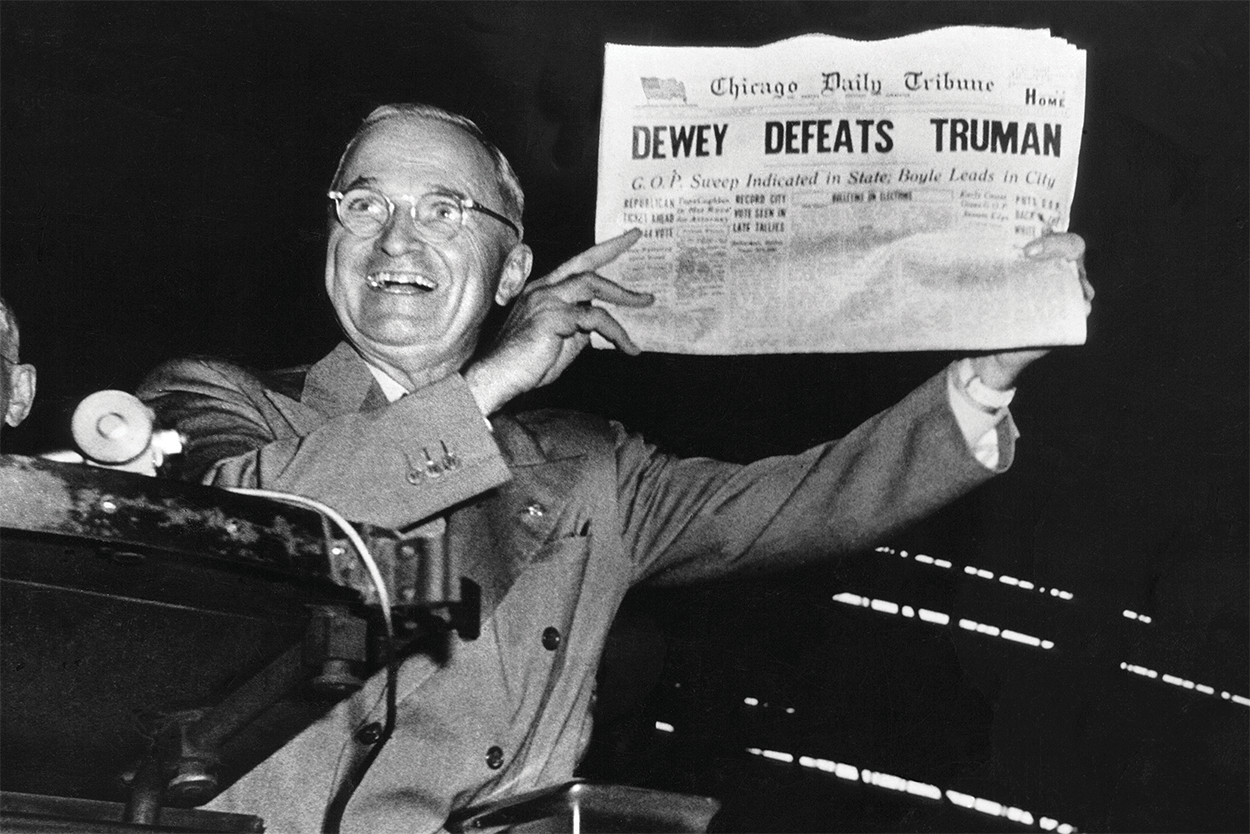
\includegraphics[width=\textwidth,height=0.7\textheight,keepaspectratio]{../../images/ch06/dewey_truman.015b2e12.jpg}
            \caption{Tác hại của Thiên kiến lấy mẫu}
        \end{figure}
    \end{columns}
\end{frame}

\begin{frame}{Sự trôi dạt Khái niệm (Concept Drift)}
    \begin{itemize}
        \item Dữ liệu Học máy không bất biến, nó thay đổi theo thời gian.
        \item \textbf{Ví dụ:} Một mô hình phân loại từ vựng IMDB năm 2011 sẽ hoạt động kém với các Review năm 2020 vì ngôn ngữ mạng đã thay đổi.
        \item \textbf{Ví dụ 2:} Gu âm nhạc, thị hiếu thời trang của người dùng thay đổi theo mùa.
        \item Đặc biệt nghiêm trọng trong Phát hiện Gian lận Thẻ tín dụng (Fraud Detection) vì các thủ đoạn lừa đảo thay đổi từng ngày.
        \item \textbf{Giải pháp:} Mô hình phải được thu thập dữ liệu và \textbf{huấn luyện lại (retrain)} liên tục.
    \end{itemize}
\end{frame}

\begin{frame}{Hiểu dữ liệu của bạn (Understanding your data)}
    Không bao giờ coi tập dữ liệu là hộp đen. Hãy trực quan hóa nó:
    \begin{itemize}
        \item \textbf{Vẽ Histogram:} Xem dải phân bố của các đặc trưng số học.
        \item \textbf{Đếm Class:} Kiểm tra xem dữ liệu có bị mất cân bằng (Imbalanced) không. Nếu có 99\% là giao dịch thường, 1\% gian lận, bạn phải có chiến lược riêng.
        \item \textbf{Rò rỉ mục tiêu (Target Leaking):} Có tính năng nào chứa "đáp án" mà ở thực tế không có không? 
        \begin{itemize}
            \item VD: Dự đoán người có nguy cơ ung thư, nhưng trong cột dữ liệu lại có thuộc tính "Đã từng hóa trị".
        \end{itemize}
    \end{itemize}
\end{frame}

\begin{frame}{Lựa chọn Độ đo Thành công (Metrics) - Balanced Data}
    Nếu không thể đo lường, bạn không thể tối ưu.
    \begin{itemize}
        \item Với dữ liệu cân bằng (Balanced data), các lớp xuất hiện đồng đều: Sử dụng \textbf{Accuracy (Độ chính xác)} và \textbf{ROC AUC}.
        \begin{equation}
            Accuracy = \frac{TP + TN}{TP + TN + FP + FN}
        \end{equation}
        \item \textit{(Trong đó: TP=True Positive, TN=True Negative, FP=False Positive, FN=False Negative)}.
    \end{itemize}
\end{frame}

\begin{frame}{Lựa chọn Độ đo Thành công (Metrics) - Imbalanced Data}
    Với dữ liệu mất cân bằng nghiêm trọng (vd: 99\% giao dịch thường, 1\% gian lận), Accuracy vô dụng (đoán bừa "không gian lận" cũng đúng 99\%). Ta phải dùng \textbf{Precision} và \textbf{Recall}.
    \begin{itemize}
        \item \textbf{Độ chuẩn xác (Precision):}
        \begin{equation}
            Precision = \frac{TP}{TP + FP}
        \end{equation}
        \textit{(Trong số các giao dịch MÁY CẢNH BÁO, bao nhiêu \% là gian lận thật?)}
        
        \item \textbf{Độ bao phủ (Recall):}
        \begin{equation}
            Recall = \frac{TP}{TP + FN}
        \end{equation}
        \textit{(Trong TỔNG SỐ gian lận có thật, máy tìm ra được bao nhiêu \%?)}
    \end{itemize}
\end{frame}

\section{3. Phát triển Mô hình (Developing a model)}

\begin{frame}[fragile]{Chuẩn bị Dữ liệu (Data Preparation)}
    \begin{itemize}
        \item \textbf{Vector hóa (Vectorization):} Mạng Nơ-ron chỉ nhận Tensor chứa số thực (float32). Mọi chữ viết, âm thanh, hình ảnh đều phải chuyển thành Tensor.
        \item \textbf{Chuẩn hóa (Normalization):} Nếu một đặc trưng chạy từ 0-1, đặc trưng khác chạy từ 100-200 sẽ làm Gradient bùng nổ. Phải đưa về $\mu=0, \sigma=1$.
    \end{itemize}
    
    \begin{lstlisting}[language=Python, caption=Cú pháp Chuẩn hóa cơ bản bằng NumPy]
# Gia su x la ma tran du lieu (samples, features)
# Tru di gia tri trung binh (Mean)
x -= x.mean(axis=0)

# Chia cho do lech chuan (Standard deviation)
x /= x.std(axis=0)
    \end{lstlisting}
\end{frame}

\begin{frame}{Xử lý Giá trị Khuyết (Handling Missing Values)}
    Nếu dữ liệu có ô bị trống (Missing):
    \begin{itemize}
        \item \textbf{Dữ liệu phân loại (Categorical):} Rất an toàn khi tạo hẳn một mục mới tên là "Khuyết" (Missing). Mô hình sẽ tự học cách xử lý nó.
        \item \textbf{Dữ liệu số (Numerical):} Không nên tự ý điền số 0 (vì có thể làm gián đoạn phân bố). Nên thay bằng \textbf{Giá trị Trung bình (Mean)} hoặc \textbf{Trung vị (Median)}.
        \item \textit{Lưu ý:} Nếu dữ liệu Test có thể bị khuyết, mà dữ liệu Train hoàn hảo, hãy cố tình "xóa" bớt một số ô trong tập Train để mô hình tập làm quen với sự thiếu sót.
    \end{itemize}
\end{frame}

\begin{frame}{Chọn Giao thức Đánh giá (Evaluation Protocol)}
    Làm sao để biết mô hình hoạt động tốt mà không chạm vào tập Test?
    \begin{itemize}
        \item \textbf{Hold-out Validation:} Dành cho dữ liệu dồi dào. Cắt hẳn $20\%$ làm Validation.
        \item \textbf{K-Fold Cross-Validation:} Dành cho dữ liệu vừa và nhỏ. Đánh giá chéo qua K vòng lặp để lấy trung bình.
        \item \textbf{Iterated K-Fold:} Lặp lại quy trình K-Fold nhiều lần với các hạt giống ngẫu nhiên (random seeds) khác nhau. Phù hợp cho dữ liệu siêu nhỏ.
    \end{itemize}
\end{frame}

\begin{frame}{Đánh bại Đường cơ sở (Beating a baseline)}
    \begin{itemize}
        \item Trước khi xây Deep Learning phức tạp, phải có \textbf{Sức mạnh Thống kê (Statistical Power)}. Tức là mô hình phải tốt hơn việc "đoán mò".
        \item Đường cơ sở (Baseline) có thể là:
        \begin{itemize}
            \item Dự đoán theo nhãn chiếm đa số.
            \item Hoặc một mô hình Học máy cổ điển siêu đơn giản (Random Forest, Logistic Regression).
        \end{itemize}
        \item \textbf{Lưu ý:} Nếu mô hình phức tạp không thắng nổi Baseline đơn giản $\rightarrow$ Giả thuyết đầu vào chứa đủ thông tin để đoán đầu ra có thể đã \textbf{SAI}.
    \end{itemize}
\end{frame}

\begin{frame}{Bảng 6.1: Chọn Activation và Loss function}
    Bạn không thể tối ưu hóa trực tiếp Accuracy hay ROC AUC (vì nó không khả vi). Phải dùng Proxy Metric là Hàm mất mát (Loss).
    
    \vspace{0.5cm}
    \resizebox{\textwidth}{!}{
    \begin{tabular}{@{}llll@{}}
    \toprule
    \textbf{Dạng Bài Toán} & \textbf{Lớp Activation cuối} & \textbf{Hàm mất mát (Loss)} & \textbf{Độ đo (Metrics)} \\ \midrule
    Phân loại nhị phân & Sigmoid & Binary crossentropy & Binary accuracy, ROC AUC \\
    Phân loại đa lớp (1 nhãn) & Softmax & Categorical crossentropy & Categorical accuracy \\
    Phân loại đa lớp (Nhiều nhãn)& Sigmoid & Binary crossentropy & Binary accuracy, ROC AUC \\
    Hồi quy vô hướng & Không có (None) & Mean squared error (MSE) & Mean absolute error (MAE) \\ \bottomrule
    \end{tabular}
    }
\end{frame}

\begin{frame}{Mở rộng Quy mô (Scaling up: Overfitting Model)}
    Để tìm ra ranh giới tối ưu, trước tiên bạn phải biết điểm Overfitting nằm ở đâu. Các bước để cố tình tạo ra mô hình Overfit:
    \begin{enumerate}
        \item Thêm các lớp (Layers) cho Mạng Nơ-ron.
        \item Tăng số lượng Nơ-ron (Units) ở mỗi lớp để tăng sức chứa (Capacity).
        \item Huấn luyện mô hình lâu hơn (tăng số Epochs).
    \end{enumerate}
    $\rightarrow$ Chú ý quan sát Training Loss liên tục giảm, nhưng Validation Loss bắt đầu tăng vọt. Ranh giới lý tưởng nằm ở chính khúc cua này.
\end{frame}

\begin{frame}{Tinh chỉnh và Chuẩn hóa (Regularizing \& Tuning)}
    Đây là bước mất thời gian nhất. Khi đã biết mô hình Overfit ở đâu, ta tiến hành gọt giũa để lấy lại hiệu suất:
    \begin{itemize}
        \item Áp dụng **Dropout** để ngắt nơ-ron ngẫu nhiên, làm cho mô hình bớt phụ thuộc vào cục bộ.
        \item Bổ sung Phạt trọng số **L1/L2 Regularization**.
        \item Thử nghiệm các siêu tham số (Learning rate, Batch size, số Units).
        \item \textbf{Cẩn thận:} Tinh chỉnh quá nhiều lần dựa trên tập Validation sẽ dẫn đến việc mô hình \textit{học vẹt} tập Validation (Information Leakage).
    \end{itemize}
\end{frame}

\section{4. Triển khai Mô hình (Deploying the model)}

\begin{frame}{Quản trị Kỳ vọng với Stakeholders}
    \begin{itemize}
        \item \textbf{Ảo tưởng AI:} Người làm kinh doanh thường hy vọng AI hoàn hảo, hiểu như con người.
        \item \textbf{Thực tế Học máy:} Mô hình chỉ khớp mẫu xác suất, luôn có sai số (False Positives, False Negatives).
        \item \textbf{Kỹ sư phải thiết lập kỳ vọng:} Không nói "Mô hình chính xác 98\%". Hãy nói: 
        \textit{"Mỗi ngày máy sẽ bắt đúng 266 giao dịch lừa đảo, chặn nhầm 200 giao dịch thật (cần nhân viên xem lại), và bỏ sót 14 giao dịch lừa đảo"}.
        \item Lựa chọn Ngưỡng xác suất (Threshold) là sự đánh đổi kinh doanh.
    \end{itemize}
\end{frame}

\begin{frame}[fragile]{Xuất mô hình (Exporting an inference model)}
    Bạn không bao giờ chạy Python Object thô trên môi trường Production. Cần xuất ra đồ thị tính toán (Computation Graph).
    
    \begin{lstlisting}[language=Python, caption=Xuất mô hình ra TensorFlow SavedModel]
# Xuat mo hinh duoi dang artifact TensorFlow SavedModel
model.export("path/to/location", format="tf_saved_model")

# Load lai o mot tien trinh khac, hoac bang ngon ngu C++
reloaded_artifact = tf.saved_model.load("path/to/location")
predictions = reloaded_artifact.serve(input_data)
    \end{lstlisting}
    
    \begin{lstlisting}[language=Python, caption=Xuất mô hình ra ONNX]
# Export theo chuan mo ONNX 
model.export("path/to/location", format="onnx")

# Load bang ONNX Runtime
ort_session = onnxruntime.InferenceSession("path/to/location")
predictions = ort_session.run(None, input_data)
    \end{lstlisting}
\end{frame}

\begin{frame}{Các Môi trường Triển khai (Deployment Environments)}
    \begin{itemize}
        \item \textbf{REST API (Cloud):} Client gửi yêu cầu HTTP, Server mạnh chạy GPU (TensorFlow Serving). 
        \begin{itemize}
            \item Ưu điểm: Mạnh mẽ. Nhược điểm: Phụ thuộc mạng, độ trễ 500ms, dữ liệu cá nhân bị gửi lên mạng.
        \end{itemize}
        \item \textbf{Trên Thiết bị (On-device / TFLite):} Chạy thẳng vào CPU di động (Android/iOS) hoặc Raspberry Pi.
        \begin{itemize}
            \item Ưu điểm: Không cần mạng, bảo mật cực cao, không trễ. Nhược điểm: Đòi hỏi mô hình phải nén siêu nhỏ.
        \end{itemize}
        \item \textbf{Trình duyệt (In-browser / TensorFlow.js):} Chạy trên máy tính người dùng bằng JavaScript.
        \begin{itemize}
            \item Tiết kiệm tiền server, tận dụng GPU cá nhân của khách hàng.
        \end{itemize}
    \end{itemize}
\end{frame}

\begin{frame}{Tối ưu hóa Suy luận (Inference Optimization)}
    Khi đưa mô hình vào các thiết bị yếu (như điện thoại), cần tối ưu kích thước:
    \begin{itemize}
        \item \textbf{Cắt tỉa trọng số (Weight Pruning):} Loại bỏ bớt các kết nối nơ-ron có trọng số quá nhỏ $\rightarrow$ Tiết kiệm RAM.
        \item \textbf{Lượng tử hóa trọng số (Weight Quantization):} Mạng Nơ-ron vốn lưu số thực chính xác kép (\texttt{float32}). Ta có thể ép nó xuống số nguyên 8-bit (\texttt{int8}).
        \begin{itemize}
            \item Kích thước giảm ngay \textbf{4 lần}.
            \item Tốc độ tính toán tăng vọt.
            \item Độ chính xác chỉ giảm cực kỳ nhỏ, gần như không đáng kể.
            \item Cú pháp: \texttt{model.quantize("int8")}
        \end{itemize}
    \end{itemize}
\end{frame}

\begin{frame}{Giám sát trên Môi trường Thực (Monitoring in the wild)}
    Ngay khi mô hình "Go Live", hiệu suất của nó sẽ bắt đầu suy giảm.
    \begin{itemize}
        \item \textbf{A/B Testing Ngẫu nhiên:} Cấp mô hình mới cho 50\% user, mô hình cũ cho 50\% user. Đo lường Doanh thu / Click-rate để chứng minh sự hiệu quả thực tế.
        \item \textbf{Kiểm toán thủ công (Manual Audit):} Chích xuất 1\% dữ liệu thực tế mỗi ngày đưa cho con người gán nhãn thủ công để so sánh với máy.
        \item \textbf{Khảo sát người dùng (User Surveys):} Nút "Báo cáo thư rác bị sai" là nguồn dữ liệu phản hồi (Feedback Loop) tuyệt vời nhất.
    \end{itemize}
\end{frame}

\begin{frame}{Bảo trì và Cập nhật (Maintaining your model)}
    Không có mô hình nào tồn tại mãi mãi do Concept Drift.
    \begin{itemize}
        \item Vòng đời của hệ thống Gợi ý nhạc có thể chỉ là vài tuần.
        \item Hệ thống Phát hiện lừa đảo thẻ tín dụng tính bằng Ngày.
        \item \textbf{Chuẩn bị cho thế hệ tiếp theo:}
        \begin{itemize}
            \item Liên tục thu thập dữ liệu sản xuất.
            \item Tìm ra những mẫu \textit{khó nhằn} mà mô hình hiện tại đang đoán sai, ưu tiên gán nhãn chúng.
            \item Retrain định kỳ $\rightarrow$ Đẩy bản cập nhật Version 2.0.
        \end{itemize}
    \end{itemize}
\end{frame}

\section{Tổng kết}

\begin{frame}{Tổng kết Chương 6}
    \begin{itemize}
        \item Machine Learning không đơn thuần là code các mạng Nơ-ron. Nó là một \textbf{vòng đời Phần mềm hoàn chỉnh (MLOps)}.
        \item \textbf{Bước 1:} Luôn định nghĩa bài toán kỹ càng, cẩn trọng với Thiên kiến dữ liệu (Sampling Bias) và chọn độ đo chuẩn.
        \item \textbf{Bước 2:} Xây dựng Baseline $\rightarrow$ Thúc đẩy Overfitting $\rightarrow$ Thu hẹp lại bằng Regularization.
        \item \textbf{Bước 3:} Đặt kỳ vọng đúng với khách hàng. Tối ưu, xuất mô hình (TFLite/ONNX) và thiết lập hệ thống giám sát liên tục (A/B Testing, Retraining).
    \end{itemize}
\end{frame}

\end{document}
